\documentclass{zusammenfassung}
\usepackage{array}
\usepackage{booktabs}
\usepackage{color}
\usepackage{colortbl}
\usepackage{xstring}
\usepackage{intcalc}
\usepackage{alphalph}
\usepackage[misc]{ifsym}
\graphicspath{ {./illustrationen/} }
\setmonofont{Linux Libertine Mono}
\usetikzlibrary{positioning}
\usetikzlibrary{matrix}

\begin{document}
\maketitle{Klasse 6/7}{07. Juli 2015}{2014/2015}

Das Ziel dieses Zirkels ist es zu sehen, wie man eine mathematische Theorie nur aus sehr wenige elementaren Grundaussagen, den
\emph{Axiomen}, aufbaut. Die Theorie, die ich mir vorgenommen habe, ist die Theorie der natürlichen Zahlen. Wir lernen rekursive
Definitionen und das Beweisprinzip der Induktion kennen und beweisen die aus der Schule bekannten Rechenregeln für die Addition
und Multiplikation natürlicher Zahlen.

Das Axiomensystem, auf dem ich aufbauen will, sind die sogenannten \emph{Peano-Axiome}. Sie bilden die in der Mathematik
übliche Art, natürliche Zahlen axiomatisch zu beschrieben.

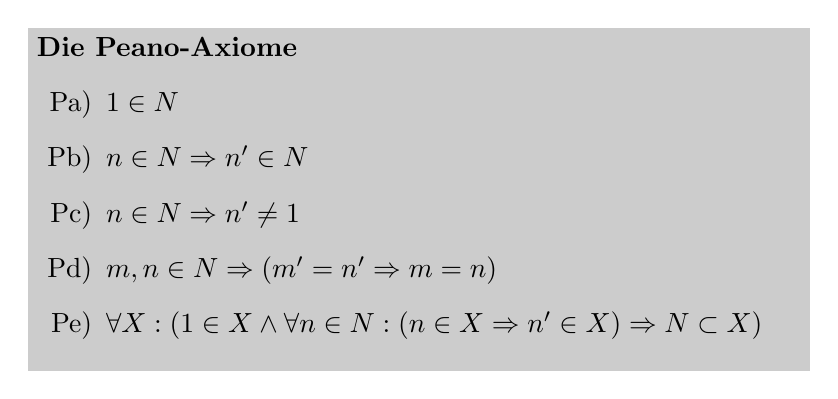
\begin{tikzpicture}
	\node[fill=black!20,rectangle] {
		\parbox{0.8\textwidth}{
			\textbf{Die Peano-Axiome}
			\begin{enumerate}
				\item[Pa)] $1\in\mathbb N$
				\item[Pb)] $n\in\mathbb N\Rightarrow n'\in\mathbb N$
				\item[Pc)] $n\in\mathbb N\Rightarrow n'\neq 1$
				\item[Pd)] $m,n\in\mathbb N\Rightarrow (m'=n'\Rightarrow m=n)$
				\item[Pe)] $\forall X:(1\in X\wedge\forall n\in\mathbb N:(n\in X\Rightarrow n'\in X)\Rightarrow\mathbb N\subset X)$
			\end{enumerate}
		}
	};
\end{tikzpicture}

Dazu sollten ein paar Worte gesagt werden. Die Notation $n'$ sollte intuitiv den \emph{Nachfolger von $n$}, also $n+1$,
bezeichnen. Wenn man diese Intuition zugrundelegt, ist es einleuchtend, dass die ersten vier Axiome für die natürlichen Zahlen
gelten sollen. Sie sagen sozusagen aus, dass der Vorrat an natürlichen Zahlen in einem gewissen Sinne groß genug ist: Ohne Axiom
Pa) könnte die Menge $\mathbb N$ leer sein. Wenn nur Pa) und Pb) gilt, könnte $\mathbb N=\{1\}$ sein, wobei dann $1$ der
Nachfolger von sich selbst wäre. Das wird durch Axiom Pc) verhindert, aber mit Pc) könnte noch $\mathbb N=\{1,2\}$ sein, wobei die
Nachfolger von $1$ und $2$ beide gleich $2$ wären. Mit Axiom Pd) ist das nun nicht mehr möglich -- dieses Axiom sagt im
Wesentlichen aus, dass die Nachfolger verschiedener Zahlen wieder verschieden sind. Jetzt haben wir erreicht, dass die Menge
$\mathbb N$ groß genug ist, um intuitiv alle natürlichen Zahlen zu enthalten.

Axiom Pe) sichert nun, dass die Menge $\mathbb N$ nicht zu groß wird. Zu Axiom Pe) sind ein paar Worte zu sagen. Erstens ist
das Zeichen $\forall(\cdots):$ einfach eine Kurzschreibweise für die Aussage "`für alle $(\cdots)$ gilt, dass \ldots"' -- wir
machen also eine Aussage über "`alle $X$"' und meinen "`alle Mengen $X$"'. Für alle Mengen $X$ soll also gelten, dass wenn $1\in
X$ ist und für alle Zahlen $n\in\mathbb N$ aus $n\in X$ auch $n'\in X$ folgt, dann sind bereits alle natürlichen Zahlen in $X$
enthalten.

Intuitiv sagt das Axiom aus, dass man jede natürliche Zahl erhält, wenn man oft genug Nachfolger von $1$ bildet. Das versetzt uns
in die Lage, Abbildungen mit Definitionsbereich $\mathbb N$ zu bilden, indem wir sagen, worauf die Abbildung $1$ abbildet, und
indem wir für das Bild von $n'$ unter der Abbildung verwenden, was mit $n$ passiert. Diese Art von Definition heißt
\emph{rekursive Definition}. Hier kommen die rekursiven Definitionen von Addition und Multiplikation:

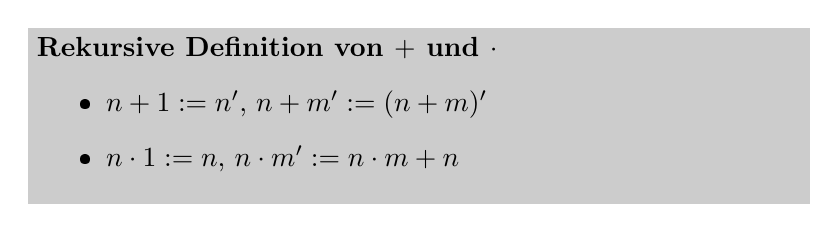
\begin{tikzpicture}
	\node[fill=black!20,rectangle] {
		\parbox{0.8\textwidth}{
			\textbf{Rekursive Definition von $+$ und $\cdot$}
			\begin{itemize}
				\item $n+1:=n'$, $n+m':=(n+m)'$
				\item $n\cdot 1:=n$, $n\cdot m':=n\cdot m+n$
			\end{itemize}
		}
	};
\end{tikzpicture}

Wenn man weiß, was Addition ist, kann man auch die Relation $<$ definieren: Eine natürliche Zahl $m$ ist genau dann kleiner als
$n$, wenn $n$ die Summee aus $m$ und einer anderen natürlichen Zahl $k$ ist, also formal
\[
	m<n:\Leftrightarrow\exists k\in\mathbb N:n=m+k.
\]
Die Schreibweise $\exists(\cdots):$ ist dabei eine Abkürzung der Aussage "`es existiert ein $(\cdots)$, sodass \ldots\ gilt"'.

Die rekursiven Definitionen von $+$ und $\cdot$ sind allerdings so unhandlich, dass es schwer ist, damit zu rechnen. Wir wollen
also die Rechenregeln beweisen, die wir aus der Schule kennen:

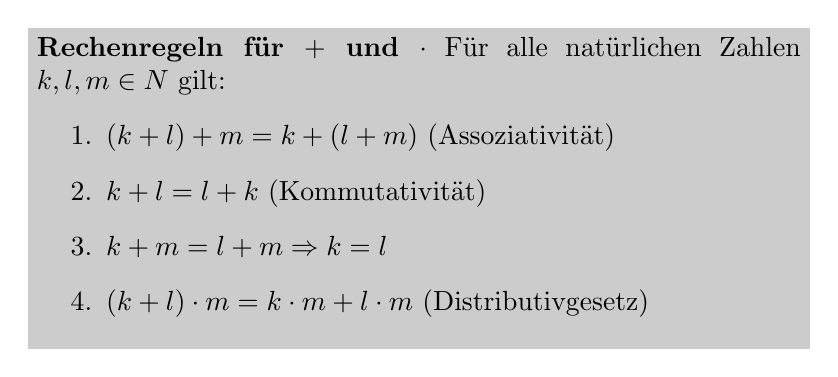
\begin{tikzpicture}
	\node[fill=black!20,rectangle] {
		\parbox{0.8\textwidth}{
			\textbf{Rechenregeln für $+$ und $\cdot$}
			Für alle natürlichen Zahlen $k,l,m\in\mathbb N$ gilt:
			\begin{enumerate}
			  \item $(k+l)+m=k+(l+m)$ (Assoziativität)
				\item $k+l=l+k$ (Kommutativität)
				\item $k+m=l+m\Rightarrow k=l$
				\item $(k+l)\cdot m=k\cdot m+l\cdot m$ (Distributivgesetz)
			\end{enumerate}
		}
	};
\end{tikzpicture}

Dabei ist es wichtig, aufzupassen, dass wir keine Rechenregeln verwenden, die wir noch nicht bewiesen haben! Die Beweise verwenden
das \emph{Beweisprinzip der vollständigen Induktion}: Die Idee dabei ist folgende: wenn man eine Aussage nur für die Zahl $1$ 
beweist und dann noch zeigt, dass aus der Richtigkeit der Aussage für $n$ auch die Richtigkeit für $n'=n+1$ folgt, dann gilt die
Aussage für alle natürlichen Zahlen. Um das formal aufzuschreiben, verwenden wir das fünfte Peano-Axiom Pe). 

Beginnen wir einmal mit Rechenregel a): Die Menge, auf die wir das Peano-Axiom anwenden wollen, ist
\[
	X:=\{m\in\mathbb N\mid\forall k,l\in\mathbb N:(k+l)+m=k+(l+m)\}.
\]
Die Schreibweise $\{\cdots\mid\cdots\}$ ist dabei eine Abkürzung für "`Die Menge aller $\cdots$, die $\cdots$ erfüllen"'. $X$ ist
also die Menge aller natürlichen Zahlen $m$, die das Assoziativgesetz mit beliebigen anderen Zahlen $k$ und $l$ erfüllen. Wenn wir
gezeigt haben, dass $X$ alle natürlichen Zahlen enthält, dann ist das Assoziativgesetz für alle Zahlen bewiesen. Wir lassen also
$k$ und $l$ in der Aussage beliebig sein und durchlaufen mit $m$ sozusagen nacheinander alle natürlichen Zahlen -- man sagt, wir
machen \emph{Induktion über $m$}.

Das Peano-Axiom Pe) gibt uns genau die Möglichkeit zu zeigen, dass $\mathbb N\subset X$ ist. Wir müssen also nur zeigen, dass die
Voraussetzungen des Peano-Axioms erfüllt sind, also $1\in X$ und $m\in X\Rightarrow m'\in X$. Zuerst $1\in X$: Das bedeutet, wir
müssen das Assoziativitätsgesetz für den Fall $m=1$ beweisen (das ist der sogenannte \emph{Induktionsanfang}). Dazu rechnen wir
einfach beide Seiten der gleichung aus:
\[
	(k+l)+1=(k+l)'
\]
und
\[
	k+(l+1)=k+l'=(k+l)'
\]
direkt aus der Definition der Addition. Daher ist die Aussage für $m=1$ wahr.

Jetzt kommt der Teil $m\in X\Rightarrow m'\in X$: Wir müssen also beweisen, dass aus der Richtigkeit des Assoziativgesetzes für
$m$ auch die Richtigkeit für $m'=m+1$ folgt. Falls $m\in X$ ist, bedeutet das, dass $(k+l)+m=k+(l+m)$ ist (diese Feststellung
nennt man die \emph{Induktionsvoraussetzung}). Jetzt rechnen wir wieder die beiden Seiten mit $m'$ ineinander um, wobei wir nicht 
nur die Definition von $+$, sondern auch das Assziativgesetz für $m$ verwenden dürfen:
\[
	(k+l)+m'=((k+l)+m)'=(k+(l+m))'=k+(l+m)'=k+(l+m').
\]
Die Induktionsvoraussetzung haben wir dabei verwendet, um $((k+l)+m)'=(k+(l+m))'$ in der zweiten Gleichheit zu erhalten. Die
Behauptung für $m'$ ist gezeigt; das nennt man den \emph{Induktionsschritt}.

Jetzt folgt aus Pe), dass $\mathbb N\subset X$ ist, und wie ich vorher schon gesagt habe, bedeutet das, dass das
Assoziativitätsgesetz für alle natürlichen Zahlen erfüllt ist.

So ähnlich funktioniert das auch bei den übrigen Rechenregeln: Bei Teil b) beweisen wir zuerst, dass immer $k+1=1+k$ gilt, und
zwar durch \emph{Induktion über $k$}.

\emph{Induktionsanfang $k=1$}: Man muss die Behauptung $k+1=1+k$ für $k=1$ nachprüfen, aber in diesem Fall sind beide Seiten ja
einfach gleich $1+1$, also stimmen sie überein.

\emph{Induktionsvoraussetzung für $k$}: Die Induktionsvoraussetzung ist die Aussage, dass die Behauptung für $k$ schon gilt, also
einfach $k+1=1+k$. Diese Gleichheit darf im Induktionsschritt verwendet werden.

\emph{Induktionsschritt}: Wir müssen die Behauptung für $k'$, also $1+k'=k'+1$, zeigen, wobei wir die Induktionsvoraussetzung
verwenden dürfen. Dazu rechnen wir
\[
	1+k'=1+(k+1)=(1+k)+1=(k+1)+1=k'+1.
\]
In der zweiten Gleichung ($1+(k+1)=(1+k)+1$) haben wir verwendet, dass wir das Assoziativgesetz schon bewiesen haben. In der
dritten Gleichung kam dann die Induktionsvoraussetzung $1+k=k+1$ ins Spiel. Der Induktionsschritt ist also bewiesen und damit ist
die Aussage für alle natürlichen Zahlen wahr.

Jetzt kommt die allgemeine Aussage $k+l=l+k$, und die wird durch Induktion über $l$ bewiesen:

\emph{Induktionsanfang $l=1$} (IA): Man muss $k+l=l+k$ für $l=1$ zeigen, aber das ist gerade die Behauptung $k+1=1+k$, die wir
schon bewiesen haben.

\emph{Induktionsvoraussetzung für $l$} (IV): Das ist die Aussage für $l$, also $k+l=l+k$. Sie darf im Induktionsschritt verwendet
werden.

\emph{Induktionsschritt} (IS): Hier müssen wir $k+l'=l'+k$ zeigen und dürfen die Induktionsvoraussetzung verwenden. Das geht so:
\[
	k+l'=(k+l)'\overset{\text{(IV)}}{=}(l+k)'=l+k'=l+(k+1)=l+(1+k)\overset{\text{a)}}{=}(l+1)+k=l'+k.
\]
In der Gleichung, über der (IV) steht, wurde die Induktionsvoraussetzung verwendet. In der Gleichung, über der a) steht, wurde
Teil a), also das Assoziativgesetz, das wir schon bewiesen haben, verwendet.

Teil c) geht wieder mit Induktion, diesmal über $m$:

(IA): Die Aussage für $m=1$ ist $k+1=l+1\Rightarrow k=l$. Da aber $k+1=k'$ und $l+1=l'$ ist, ist das nichts anderes als das
Peano-Axiom Pd).

(IV): Für den Beweis des Induktionsschritts darf man $k+m=l+m\Rightarrow k=l$ verwenden.

(IS): Wir müssen zeigen, dass aus $k+m'=l+m'$ folgt, dass $k=l$ ist. Es gilt $k+m'=(k+m)'$ und $l+m'=(l+m)'$, das heißt, aus
$k+m'=l+m'$ folgt mit Pd), dass $k+m=l+m$ ist. Jetzt kann man die Induktionsvoraussetzung anwenden und erhält $k=l$ wie gefordert.

Teil d) geht wieder mit Induktion über $m$.

(IA): Für $m=1$ ist die Aussage $(k+l)\cdot 1=k\cdot 1+l\cdot 1$. Da Multiplikation mit $1$ per Definition nichts macht, sind
beide Seiten gleich $k+l$ und stimmen daher überein.

(IV): Für (IS) darf $(k+l)\cdot m=k\cdot m+l\cdot m$ verwendet werden.

(IS): Hier rechnet man ein bisschen vor sich hin, wobei sowohl die Induktionsvoraussetzung (IV) als auch die Assoziativität und
die Kommutativität -- also a) und b) -- verwendet werden:
\begin{align*}
	k\cdot m'+l\cdot m'&=(k\cdot m+k)+(l\cdot m+l)\overset{a)}{=}((k\cdot m+k)+l\cdot m)+l\\
																			 &\overset{a)}{=}(k\cdot m+(k+l\cdot m))+l\overset{b)}{=}(k\cdot m+(l\cdot m+k))+l\\
																			 &\overset{a)}{=}(k\cdot m+l\cdot m)+(k+l)\overset{(IV)}{=}(k+l)\cdot m+(k+l)=(k+l)\cdot m'
\end{align*}
Damit ist der Induktionsschritt gezeigt und das Distributivgesetz für alle Zahlen bewiesen.

\begin{aufgabe}
	Beweise die folgenden übrigen drei Rechenregeln: Für alle natürlichen Zahlen $k,l,m\in\mathbb N$ gilt:
	\begin{enumerate}
			\setcounter{enumi}{4}
		\item $k\cdot l=l\cdot k$
		\item $k\cdot(l+m)=k\cdot l+k\cdot m$
		\item $(k\cdot l)\cdot m=k\cdot(l\cdot m)$
	\end{enumerate}
\end{aufgabe}

\begin{aufgabe}
	Finde eine rekursive Definition für Potenzen $n^m$ natürlicher Zahlen!
\end{aufgabe}

\begin{aufgabe}
	Die \emph{Fakultät} $n!$ einer Zahl $n$ ist das Produkt der Zahlen von $1$ bis $n$. Gib eine rekursive Definition für die
	Fakultät an!
\end{aufgabe}

\begin{aufgabe}
	Finde eine formale Definition dafür, dass $m$ ein Teiler von $n$ ist (ähnlich zu der Definition der Relation $<$). Man schreibt 
	kurz $m|n$ dafür, dass $m$ ein Teiler von $n$ ist.
\end{aufgabe}

\begin{aufgabe}
	Zeige mit vollständiger Induktion, dass $n^5-n$ für alle natürlichen Zahlen $n\in\mathbb N$ durch $5$ teilbar ist.
\end{aufgabe}

\begin{aufgabe}
	Zeige mit vollständiger Induktion, dass $5^{2n}-2^n$ für alle natürlichen Zahlen $n\in\mathbb N$ durch $23$ teilbar ist.
\end{aufgabe}

\end{document}
